%----------------------------------------------------------------------------
\chapter{Megoldási lehetőségek}
\label{sec:solutions}
%----------------------------------------------------------------------------

Ebben a fejezetben szeretném bemutatni, hogy a korábban \aref{sec:results} fejezetben látott mérések alapján milyen megoldási lehetőségek jöhetnek számításba.
Természetesen minden bemutatott megoldásnak megvan a saját erőssége és gyengesége, amiket a következő alfejezetben részletesen is ismertetek.

%----------------------------------------------------------------------------
\section{Feltárt probléma rövid összefoglalása}
%----------------------------------------------------------------------------

A megoldási lehetőségek bemutatása előtt szeretném röviden  a problémát és felvetést, amire keressük a megoldást.
A mérési eredmények alapján arra jutottam, hogy léteznek olyan skálázási helyzetek, amikor a Kubernetes jelenlegi skálázója nem tud ideálisan lekezelni.
Ez a működés onnan fakad, hogy a futó alkalmazásról nem rendelkezik globális ismerettel, csak az egyes független szolgáltatásokat kezeli a többitől függetlenül.

A látott mérésekből kiderült, hogy a jelenlegi rendszerben létezik egy átbukási pont, amikor a beérkező kéréseket az össz alkalmazás már nem képes időben kiszolgálni, mert az egyik szolgáltatási komponens túlterhelt állapotba kerül.
Ilyenkor a beérkező kérések továbbra is fogadásra kerülnek és elkezdődnek a pufferek megtöltései a rendszerben.
Ez egy öngerjesztő folyamatot indít meg, ahol a hosszabb sorbaállás, a folyamatos túlterheltség miatt aránylag egyre kisebb lesz a sikeres kiszolgálások száma. 

A hatékonytalan működésen az sem segít, hogy az előre beállított idő túllépése után bontjuk a kapcsolatot, azonban ezt az alkalmazás nem tudja lekezelni.
Nem létezik implementált megoldás arra az esetre, hogy az ilyen kérések által keltett az egyéb alkalmazás egységek terhelését megszüntesse.
Értelemszerűen ebben az esetben felesleges még a back-end oldalán elvégezni az erőforrás intenzív feladatot, amikor az azt kiváltó eredeti kérés eldobásra került.

A feltárt problémát két részre lehet osztani, amik egymás hatását tudják erősíteni vagy gyengíteni.

%----------------------------------------------------------------------------
\section{Lehetséges eszközök}
%----------------------------------------------------------------------------

A kiírásban megfogalmazott feladatom volt, hogy keressek olyan kiegészítést vagy javaslatot, ami a jelenlegi HPA működését javítani tudná.
A feladatom elvégzése és források keresése közben számos megoldási lehetőség felmerült.
A bemutatott eszközök elemzése során látni fogjuk, hogy kicsit más megközelítésből és a probléma más aspektusát célozva próbálja a feltárt hatásokat csökkenteni.

Az egyes eszközök értékelésénél az is fontos szempont volt, hogy a lehető legkevesebb módosítást kelljen végrehajtani az alkalmazás oldalán.
Ez fontos, mert a megvalósítani kívánt feladat nem tartozik szorosan az alkalmazáshoz és ideális esetben teljesen transzparens módon működne.
Természetesen több dolgot is mérlegelni kell az adott helyzetben ideálisnak ítélt megoldás kiválasztása közben.

Fontos azt is megfontolni, hogy egy az infrastrukturális részekre hatást gyakorló eszköz milyen információk alapján engedjük, hogy dolgozzon.
Természetesen minél több információval rendelkezünk az adott alkalmazást illetően, annál optimálisabb megoldásokat tudunk adni.
Például, ha egy okos skálázónak rálátást adunk az alkalmazás hálózatára, az egyes egységek által használt erőforrásokra, a köztük lévő kapcsolatra és esetleg saját metrikákat is kivezetünk, akkor a skálázási döntés meghozatalában ezeket mind számításba tudjuk venni.
Másik oldaról viszont aggályos lehet, ha ilyen szintű monitorozást és belelátást biztosítunk, mert ezáltal következtetéseket tudunk levonni a futtatott alkalmazásról.
Ez pedig bizonyos esetekben az ügyfél érdekeit sértheti.


\subsection{Beépített állapotjelzők}
%----------------------------------------------------------------------------
A Kubernetes kapszulák létrehozása közben, beépített módon lehetőségünk van a kapszula állapotáról jelzési pontokat meghatározni.
Ezzel a megoldással sokrétűen használható funkciókat kapunk, amivel közvetetten több dolog befolyásolására nyílik lehetőségünk.
Három jelzési módszerünk van, amit három különböző esetre találtak ki.
Az alapvető felvetés onnan fakad, hogy különböző, gyakran előforduló helyzetekre adnak megoldási lehetőségeket különálló működésük által.
Az egyes állapotjelzők ideális használati módját az alábbi szituációkkal szeretném szemléltetni.

\begin{enumerate}
    \item \textbf{(Liveness probe - életteli próba)} Előfordulhat, hogy az alkalmazásunk valamilyen bemenetek következtében holtponti állapotba kerül, amit nehéz lenne kívülről észrevenni, viszont külső behatás nélkül nem tudna továbblépni belőle. 
    Illetve egyéb okok miatt is kerülhet olyan állapotban, amikor a vizsgált alkalmazás nem képes ellátni a működését, mindezt különösebb hiba és kilépés nélkül teszi.
    Szerencsére az ilyen esetek nem számítanak különösnek és hamar fel is lehet oldani az egység újraindításával, amit az életteli próbával tudunk kezelni.
    Ez egy teljesen ideális implementáció esetén nem fog gondot okozni, hiszen a kapszulák nem tartalmaznak, tárolnak fontos adatokat és állapotokat.
    Egy újraindítás sokkal idő- és költséghatékonyabb megoldás, mintha az egész rendszer funkcionális működését veszélyeztetnénk.

    \item \textbf{(Startup probe - indítási próba)} Eshetőség, hogy az alkalmazás elindítása után még el kell végezni pár inicializációt, mielőtt a külső kérések kiszolgálását elkezdhetné.
    Ebben az esetben is tudatni kell az infrastruktúra részére, hogy a jelenlegi állapotába még nem áll készen a működésre.
    Nagy hibázási lehetőséget rejtene magába, ha erre a korábban látott  életteli próbát használjuk, mert nehéz kiszámítani mennyi időt fog igénybe venni a komponens elindulása.
    Külön emiatt létezik az indítási próba, ami csak akkor fogja az adott kapszula állapotát készenléti státuszba sorolni, ha sikeresen lefutott a próba.

    \item \textbf{(Readiness probe - készenléti próba)} Tegyük fel, hogy van egy szolgáltatásunk, ahol nagy fájlok feltöltésére van lehetőségünk.
    A megvalósított funkció szám
    Ez egy időigényesebb feladat lesz, miközben az alkalmazásunkat nem szeretnénk további kérésekkel terhelni.
    Ebben az esetben meg kell várni a korábban érkező kérés kiszolgálását és csak utána van lehetőségünk fogadni a többit.
    Ilyen helyzetben tudjuk használni a készenléti próba jelzést. 
    Amennyiben a próba sikertelen vol, tehát jelenleg nem engedhetünk új kiszolgálást, akkor a kapszula IP címe ki fog kerülni erre az időszakra a hozzá tartozó \textit{Service} alól, így forgalom se fog eljutni hozzá. 
    
\end{enumerate}

A fentebb bemutatott eszközök megkönnyítik a robusztus rendszerek építését.
Segítségükkel kihasználhatjuk, hogy inkább az előforduló hiba gyors észrevételét és nem annak az elkerülését részesíti előnyben.
Erre lehetőség is van, mert az új konténerek elindítása általában pár másodperc alatt megtörténik és ezáltal egy öngyógyító tulajdonsággal is fog bírni a kész rendszer.
Így pedig a rendszer megbízhatósága is javulni fog. 

Ennek ellenére körültekintően kell ezeket az eszközöket is használni, hiszen rossz konfiguráció esetén mi magunk tehetjük működésképtelenné a rendszert.
Például, hibás beállítás esetén az életteli próba hajlamos állandóan újraindítani az alkalmazást. Vagy a készenléti próba miatt egyes komponens egységek nem fognak annyi kérést kapni, amit azok valóban képesek lennének kiszolgálni.

\subsubsection{Módszer tesztelése}
A következő feladat az volt, hogy a bemutatott állapotjelzők használatával ismét el kellett végezni a korábbi mérést és megnézni az elért hatását.
Számomra a készenléti probléma volt a legérdekesebb, hiszen ez a megoldás ad lehetőséget arra, hogy addig ne érkezzen kiszolgálandó kérés az adott alkalmazás egységhez, amíg egy bizonyos állapot teljesül.

A mérés elvégzéséhez fel kellett készíteni a korábban megírt operátort, hogy a \textit{Deployment} létrehozása közben egy készenléti próba definíciót is építsen bele. 
Valamint minden egyes alkalmazásegységnek rendelkeznie kell egy olyan végponttal, ami nem jelent számottevő többlet terhelést, és az ide érkező kérések kiszolgálása alapján tudja megmondani a rendszer jelenlegi terheltségét. 
Amennyiben a próba sikertelen, tehát a rendszer túlterhelt állapotban van, akkor nem szabad számára több kérést továbbítani, amíg nem csökken a kiszolgálásra váró kérések sora.

% MultiFE & SingleBE with Readiness probe -------------------------------------------------------
\begin{figure}[!ht]
\centering
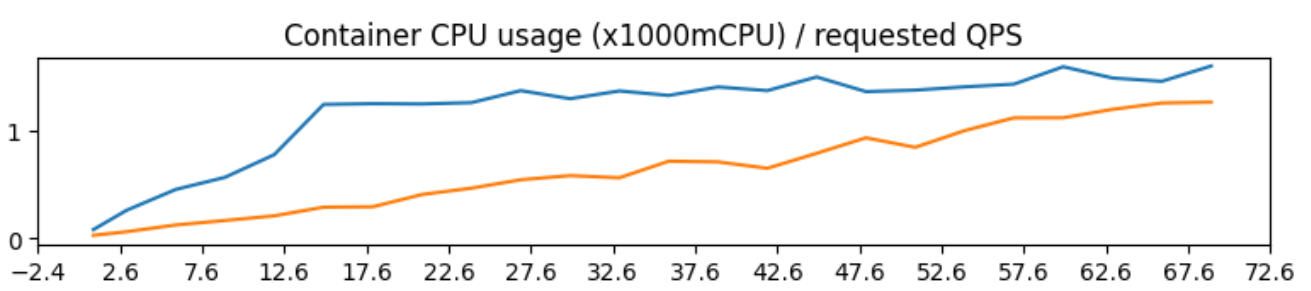
\includegraphics[width=150mm, keepaspectratio]{figures/multiFE-singleBE-readinessprobe.png}
\caption{Korábbi szimuláció megismétlése készenléti próbával}
\label{fig:readiness-probe-measurement}
\end{figure}

A módszer hatékonyságának vizsgálata érdekében arra gondoltam, hogy egy korábban már bemutatott mérést fogok megismételni, csak kibővítve az állapotjelzővel.
Ehhez \aref{fig:todo} mérést választottam.
A szimuláció elvégzését követően kapott eredmények sajnos nem váltották be a hozzájuk fűzött reményeket, és nem javultak számottevő mértékben a kiszolgálási paraméterek.
Összességben hasonló tendenciát lehetett megfigyelni, mint a korábbi, próba nélküli mérés esetén. 
A mérés elején folyamatosan emelkedett a kiszolgált kérések száma, azonban az eredeti méréssel azonos időben és helyen megindult a meredek visszaesés is.
Ez amiatt lehetett, mert a beérkező kérések kiszolgálása továbbra sem tudott megtörténni az öt másodperces időkorláton belül.
Emiatt nem szeretném részletekbe menően elemezni minden korábbi eredményt, egyedül az említésre-méltó processzorfelhasználást.
A kapott értékeket \aref{fig:readiness-probe-measurement} ábra tartalmazza.
Az eredeti méréssel azonos tendenciát figyelhetünk meg. 
Ebben az esetben is azt látjuk, hogy a backend CPU felhasználása hamar egy plafonba ütközik, amin túl kitörni már nem tud.
Illetve ezzel párhuzamosan a költséghatékony frontend továbbra is fogadja a beérkező kéréseket, ami miatt további erőforrásokat fog elhasználni.
Emlékezzünk, hogy a korábbi méréseknél a backend részére 2000 mCPU és a frontend kapszuláknak pedig 1000 mCPU limitáció volt beállítva.
Ezen limitek a mostani méréseknél sem változtak, azonban az ábráról tisztán leolvasható, hogy a felhasznált erőforrás mennyisége a korábbitól jelentősen elmaradt.
Azt láthatjuk, hogy a beállított próba hatására a backend és a frontend által elhasznált erőforrások mennyisége lecsökkent.
Az lehet erre a magyarázat, hogy a backend, amikor érzékelte, hogy kezd túlterhelődni, akkor egy kisebb időszakra szüneteltette a kérések fogadását, ami miatt arányaiban csökkent a mérések során elhasznált processzor mennyisége.

Sajnos azonban a beállított próbával sem sikerült elérni, hogy a kiszolgálási mutatók megfelelő mértékben javuljanak, hiszen a megismételt mérésben is egy megadott pont után visszaesett a sikeres kiszolgálások száma. Jelen állásban minden alkalmazás egység saját magának a terheltségét tudja monitorozni, ami miatt hiába van a sor végén lévő backend komponens leterhelve, ezt a frontend még nem érzékeli és továbbra is fogadni fogja a felé irányított kéréseket.
Esetleg érdemes lehet további finomításokat bevezetni és egy saját szkripttel ellenőrizni a láncolat végén elhelyezkedő backend állapotát a frontend oldaláról is.
Ezzel megoldhatóvá válna, hogy a lassú komponenshez igazodva tudjuk a kéréseket fogadni már a kiszolgálási lánc elején.

Természetesen a vázolt megoldás is tartalmaz néhány kifogásolható aspektust. 
Az ilyen módon összeállított rendszer egy másik komponens állapotát monitorozza és ez alapján tudja a saját készenléti állapotjelzőjét állítani. 
Statikusan kell ezen próbákat beállítani és a terhelés változásával változhat a szűk keresztmetszet is.
Például egy valódi forgalmat elemezve rendszeresen megjelenik, hogy periodikusan lesznek terhelve a komponensek.
Nap elején elképzelhető, hogy a bejelentkeztető komponens lesz túlterhelt és szűk keresztmetszet, míg nap közben pedig az adatok validációjáért felelős szolgáltatás.
Ezen változásokat pedig nehéz lehet lekezelni, egy egyszerűbb szkripttel.


\subsection{Konténer specifikus metrikák alapján}
\label{subsec:container_metric_scaling}
%----------------------------------------------------------------------------
Következőnek ismertetett megoldási javaslat szintén a beépített Kubernetes erőforrásokat és azok funkcióit kívánja felhasználni.
Ezen megoldásoknak előnye, hogy a klaszter oldaláról nem igényelnek nagy mértékű többlet fejlesztést és támogatást, hiszen ezek a funkciók valószínűleg rendelkezésre állnak már a rendszerben vagy pedig könnyen telepíthetőek.
A mérleg másik oldalán ezen megoldások az alkalmazás oldalán igényelnek fejlesztéseket vagy pedig a helyes konfiguráció okozhat kihívást.

Még korábban, \aref{subsec:hpa} alfejezetben bemutatott HPA skálázás esetén említésre került, hogy tetszőleges metrikák alapján is lehetőségünk van skálázni.
Alapértelmezetten és leginkább a mérések által általunk is használt processzor erőforrás igény alapján történő skálázás a legelterjedtebb forgatókönyv.
Ezen metrikákat a klaszter automatikusan tudja gyűjteni, így a skálázók konfigurációja és elindítása egyszerű folyamattá tud válni.
Illetve a legtöbb esetben, ha a klaszterünkben nincsenek szűkös erőforráshatárok aránylag jó működést eredményez.

A megoldási lehetőség hátránya, hogy ezen implementáció is lokálisan az egyes alkalmazásegységek skálázását fogja végezni.
Így pedig, amikor az erőforrások allokációja nagymértékű nem képes a rendszer áteresztőképességét figyelembe venni.

Továbbá nincs a skálázás mögött egy dinamikus algoritmus.
Továbbra is az indítás pillanatában beállított konfigurációk alapján fogja meghozni a skálázó a döntéseit.
Emiatt a kezdeti konfigurációnál nagyon alaposan végig kell gondolni, hogy milyen szabályokat szeretnénk alkalmazni.
Esetlegesen rosszul felmért metrikák alapján többlet erőforrásokat is lefoglalhatunk a kiszolgálási metrikák javulása nélkül.

A megoldás felvetése, hogy az alkalmazás logikai rétegében legyenek követve, mentve és exportálva olyan metrikák, amik az alsóbb-szintű infrastruktúra réteg döntéseinek lesz az alapja.
Ezt szintén mérlegelni kell, hiszen nem tartozik szorosan az alkalmazás logikai részéhez illetve bizonyos mértékű többlet fejlesztést is igényel.

\subsection{Szolgáltatás hálók által nyújtott lehetőségek}
%----------------------------------------------------------------------------
Több új kihívás is megjelent a mikroszolgáltatások elterjedésével, amivel szembe kellett nézni a fejlesztőknek és az üzemeltetőknek is.
Ezen kihívások mentén született meg a szolgáltatás hálók (\textit{service mesh}) fogalma. 
Fontos megjegyezni, hogy a fejezetben tárgyalt szolgáltatás háló kifejezés a dolgozatban szereplő többi előfordulásán túl egyéb megkötéseket is tartalmaz.
Emiatt szeretném tisztázni, hogy a következőkben használt szolgáltatás háló alatt mit értünk.

A szolgáltatás háló egy lehetséges módja, hogy szabályozzuk az alkalmazásrészek közti kommunikációt. 
Általa egy külön infrastruktúra réteget tudunk létrehozni, amin keresztül láthatjuk és szabályozhatjuk a komponensek közti kommunikációt.
Ezzel ígéretet kapunk a kommunikáció optimalizációjára, amivel együtt az esetleges kieséseket is csökkenthetjük\citep{serviceMeshDefinition}.

Az egyes alkalmazás komponenseket nevezzük egy-egy szolgáltatásnak, és az ő kommunikációjuk által alkothatunk belőlük hálózatot.
Több megvalósítás is létezik, azonban a felépítésük nagyon hasonlít.
Egy ilyen architektúra bemutatása látható \aref{fig:serviceMesh-topology} ábrán.

Az ábrán \textit{Instance A/B/C} névvel ellátott alkalmazás egységek valósítanak meg egy-egy szolgáltatást az elképzelt mikroszolgáltatás architektúrában. 
Jól látható, hogy köztük nem történik semmilyen közvetlen kommunikáció, csak a mellettük lévő oldalkocsival (\textit{sidecar}) vannak kapcsolatban.
Ezek az oldalkocsik tipikusan egy konfigurálható proxyt tartalmaznak és az adott szolgáltatás mellett üzemelnek.
Ezt a mintát nevezik a oldalkocsis mintának (\textit{sidecar pattern})\citep{sidecarPattern}.
Minden, a szolgáltatások által küldött és fogadott kérésnek keresztül kell menni ezen a proxyn, ami pedig így belelátást kap a csomagokba illetve azok továbbítására is ráhatása van.
Ezáltal nyomon követhető és megfigyelhető lesz a komponensek közti kommunikáció.
Ez önmagában is előnyös, hiszen könnyebben meg lehet tudni, hogy az egyes szolgáltatáshálók milyen kiszolgálást tudnak nyújtani, könnyebb kideríteni az aktuálisan legszűkebb keresztmetszetet.
Természetesen a rendszerbe kötött proxykat kezelni is kell, amire egy külön réteg van, azonban ez már nagyobb mértékben specifikus az egyes megvalósításokra.


% Service Mesh Topology -------------------------------------------------------
\begin{figure}[!ht]
\centering
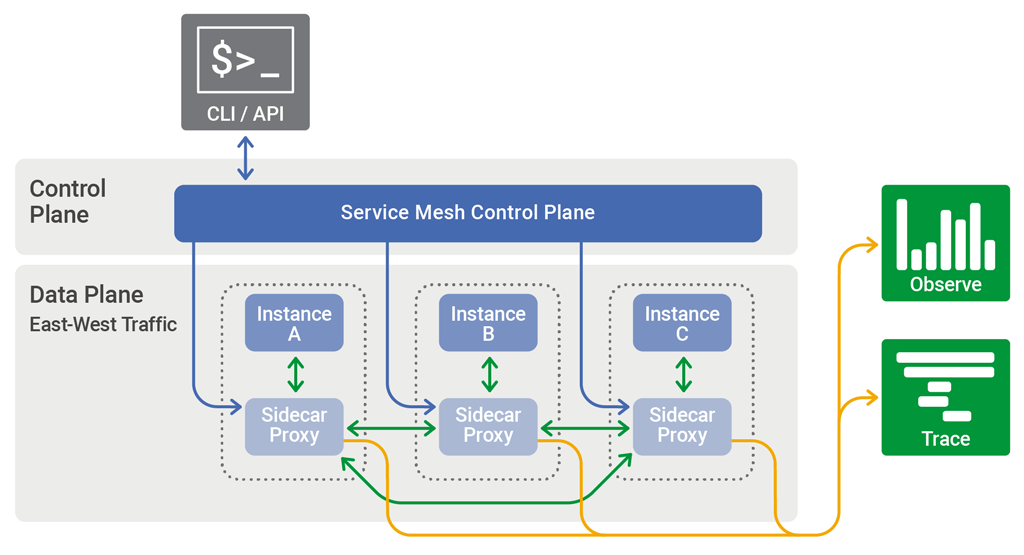
\includegraphics[width=150mm, keepaspectratio]{figures/service-mesh-generic-topology.png}
\caption{Szolgáltatás hálót alkotó komponensek és működésük\citep{serviceMeshTopology}}
\label{fig:serviceMesh-topology}
\end{figure}

Az új architektúra is rendelkezik bizonyos megkötésekkel, amit az alkalmazása előtt figyelembe kell venni.
Mivel új komponenseket hozunk be a kommunikációba, ezért a késleltetések is meg fognak nőni.
Valamint a proxyk működtetése is többlet erőforrásokkal fog járni. 
Természetesen növelni fogja a processzor foglaltságot és használtságot, valamint az alkalmazás futtatásához memóriára lesz szükség.
További hátránya, ami egyben az előnye is, hogy egy új komplexitást hoz be az amúgy is összetett alkalmazás üzemeltetésbe. 
Ezért az architekturális döntés meghozatalában körültekintően kell eljárni.


\subsubsection{Gloo Edge}
%----------------------------------------------------------------------------
- Ingress controller - hivetkozás
- Mivel tud kevesebbet, mint a service mesh

\subsection{Okos skálázó}
%----------------------------------------------------------------------------

A korábban bemutatott megoldási lehetőségeknél, \ref{subsec:container_metric_scaling} alfejezetben látottat leszámítva, a fő motiváció a beérkező terhelés szabályozása volt.
Az eredeti problémánkat viszont több irányból is meg lehet fogni.
Másik megközelítésben az erőforrások globálisan optimális elosztása a fő szempont a megoldandó kihívás.

A következő megoldási javaslat ezt a megközelítést veszi alapul és bővíti ki a korábban látott javaslatokkal.
A javaslat egy központi skálázó alkalmazás, ami folyamatosan monitorozza a klaszter teljes állapotát és az éppen futtatott alkalmazásokat is.
A skálázási javaslatokat pedig ezen információk összességéből tudja meghatározni.
Így figyelembe tudja venni az egyes kapszulák minőségi osztály besorolásuktól kezdve az egyes komponensek közti forgalmak megosztásán keresztül az esetlegesen exportált alkalmazás metrikákig.

Ezzel a megoldással lehetőségünk lenne az alkalmazás egységek kezelése helyett a teljes rendszer számára ideális döntéseket meghozni.
Akár több névtérben futó rendszerek erőforrás allokációit is össze lehet hangolni, ami további optimalizálást jelentene.

A bemutatott javaslatok közül ez a megoldás a legkomplexebb is. 
Ez egyértelműen a Kubernetes platform nyílt forráskódjának bővítésével járna.
Egy ilyen projekt jelentős szakmai erőforrás ráfordításával járna, hiszen az újfajta skálázóhoz új erőforrásokat is létre kell hozni illetve a kezeléshez szükséges logikát implementálni is kell.

Nem elhanyagolható felvetés, hogy a skálázási algoritmus logikájának bonyolítása jelentős kockázatokkal járhat, ha annak paraméterezését a felhasználóra bízzuk.


\subsection{HPA és VPA skálázó}
%----------------------------------------------------------------------------
%Az alapképzés végén készített szakdolgozatom 

%Az okosított skálázó hátrányainál is szerepel, hogy igazán specifikus működést csak kellően nagyszámú konfigurációval lehet elérni, ami vis

%Namespacek között

%fejlesztés, tesztelés

%pl: nyomon követi milyen arányban használják az erőforrásokat

%Amdahl's törvényt is figyelembe  veszi
%VPA és HPA együtt működik
%Szimulációk futtatására is ideális a rendsezr